\documentclass[12pt]{standalone}
\usepackage{tikz}


\begin{document}
\begin{tikzpicture}
    \fill[red!75]\foreach \a in
        {(0,0), (2,0), (4,0), (2,1), (4,1), (0,2), (1,2), (3,2), (2,3), (4,3), (0,4), (1,4), (3,4)} 
        {\a rectangle +(1,1)};
    \fill[blue!75]\foreach \a in 
        {(1,1), (2,2), (3,3), (4,4), (5,5), (3,1), (5,1), (4,2), (1,3), (5,3), (2,4), (1,5), (3,5)} 
        {\a rectangle +(1,1)};
    \draw[gray, line width=0.6mm] (0,0) grid (6,6);
    \draw[black, line width=0.6mm] (0,0) rectangle (6,6);
    \node at (11,3) {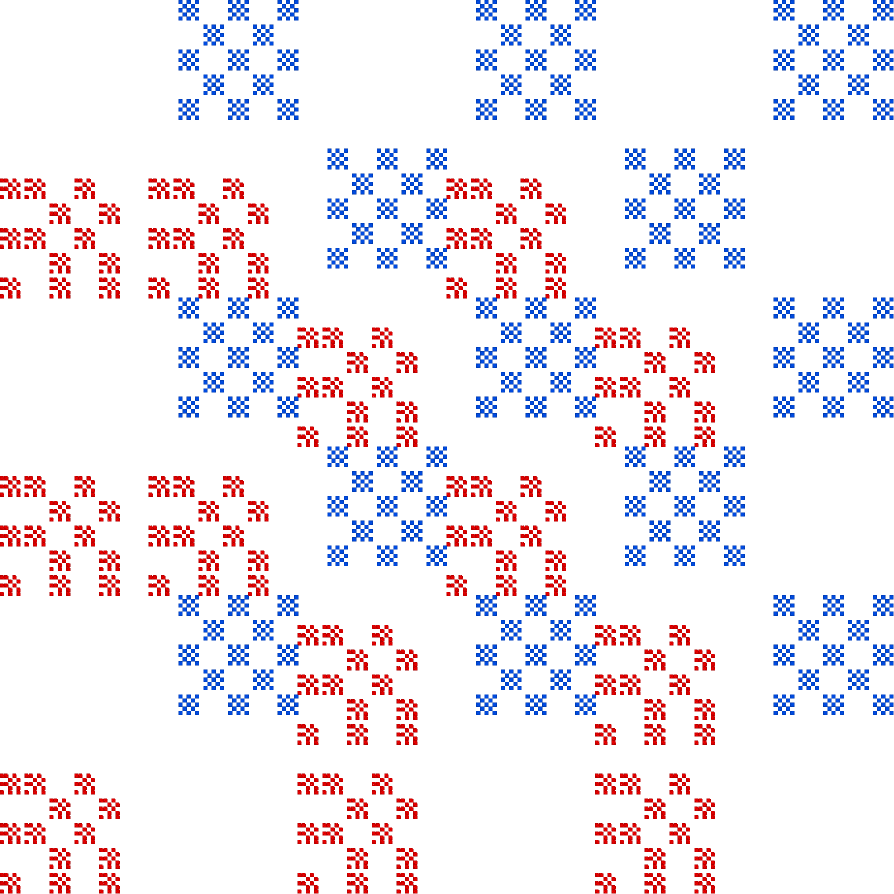
\includegraphics[width=6cm]{FSI_6x6_K.png}};
    \fill\foreach \a in
        {(2,1), (4,1), (3,2), (2,3), (4,3), (3,4)} 
        {\a++(8,0.333) circle (0.08) \a++(8,0.666) circle (0.08)};
	\fill\foreach \a in
        {(1,2), (3,2), (2,3), (4,3), (1,4), (3,4)} 
        {\a++(8.333,0) circle (0.08) \a++(8.666,0) circle (0.08)};
\end{tikzpicture}
\end{document}
% FSI_6x6_DS